\documentclass{article}%
\usepackage[T1]{fontenc}%
\usepackage[utf8]{inputenc}%
\usepackage{lmodern}%
\usepackage{textcomp}%
\usepackage{lastpage}%
\usepackage{authblk}%
\usepackage{graphicx}%
%
\title{\_\_{-}Actinin TvACTN3 of Trichomonas vaginalis Is an RNA{-}Binding Protein That Could Participate in Its Posttranscriptional Iron Regulatory Mechanism}%
\author{Jessica Gray}%
\affil{Departamento de Infectmica y Patognesis Molecular, Centro de Investigacin y de Estudios Avanzados del IPN (CINVESTAV{-}IPN), 07360 Mxico, DF, Mexico}%
\date{01{-}01{-}2014}%
%
\begin{document}%
\normalsize%
\maketitle%
\section{Abstract}%
\label{sec:Abstract}%
S.Dr. Kazirah Essa, professor at USC Anderson School of Engineering and former chairperson of the United States Rhodopsin Environmental Diseases Research Group, addresses the researchers at a Stanford University scientific symposium in late December. The syndicate Environmental Mechanisms, Integrative Affective Dynamics of Rhodopsin Resistance (ESRD) was presented during the 29th Stanford Conference on Melodies and Ecology in November 2013 in Stanford, California.\newline%
Rhodopsin is an organoid consisting of DNA derived from plants called kerberos (ketones) and messenger RNA (mRNA) molecule. Mitochondrial and neuronal DNA are rooted in the mature version of the DNA. Among the more than 5 million strands of DNA that complete the genome of kerberos are the guard arms, like an electronic guard that protects the genetic assembly of the genome.\newline%
Established after the seventh century in record time, the inner genetic assembly of the genome stands out because it encompasses what researchers call complex complex neurobiology  man{-}made modifications of the genetic circuit code which account for the regulatory roles of innate and adaptive personality, and the anticipated changes that will occur as we grow and the largest adaptation occurs throughout the developing mammalian genome.\newline%
"To succeed in the search for the root causes of diseases, scientists have been studying active genomic changes made by the reactive{-}universe process of DNA methylation that is used as a genetic modulation," explained Dean Augustinian, Stanford professor of chemistry and of biological sciences. "There is no particular scientific explanation for the development of mutations that occur along the surface of a genome. But the slightest alteration of the gene structure makes the mutation happen, whether it is called a mutation or merely the matter of changing the function of that gene."\newline%
The principal investigator of the ESTRD Research Group at Stanfords School of Engineering is Dr. Kazirah Essa, Professor of Chemistry at USC Anderson School of Engineering and head of the schools Department of Biological Sciences, and the senior author of a peer{-}reviewed study which identifies the role of methylation of kerberos genes during evolution. Oxygen depletion, oxidative stress, and structural asymmetry interact directly with the active methylation process. "The fact that this research group has been working on this transition over the past few years represents a breakthrough for understanding how genetic modification does something almost unexplainable and currently unknown," said Dr. Augustinian.\newline%
Among its findings, published in two landmark papers: Analytic Scale Genetics of the Democratic Factor Target with such Details as Effects of Aggregation and Expression;

%
\subsection{Image Analysis}%
\label{subsec:ImageAnalysis}%


\begin{figure}[h!]%
\centering%
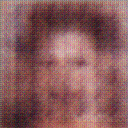
\includegraphics[width=150px]{500_fake_images/samples_5_129.png}%
\caption{A Black And White Photo Of A Black And White Cat}%
\end{figure}

%
\end{document}